%************************************************
\chapter{Aprendizaje Automático}\label{ch:ML}
% ************************************************
%--- Deep Learning Ian G book
% Historical dev
% big data &  improve of memorie in computer
% poner el puto diagramita q siempre sale
\begin{flushright}{\slshape
    El aprendizaje automático es como una caja de bombones: nunca sabes lo que vas a obtener... a menos que tengas buenos datos y una sólida comprensión de tus algoritmos.} \\ \medskip
    --- ChatGPT AI language model
\end{flushright}



La \textbf{Inteligencia Artificial}, o AI por sus siglas en inglés, se puede definir como un sistema capáz de interactuar con su entorno. Algunos ejemplos de Inteligencias Artificiales son: \emph{Siri} de Apple y \emph{Alexa} de Amazon. Para poder generar una respuesta al entorno, estos sistemas contienen sensores que permiten la entrada de información, en estos ejemplos la información es obtenida mediante la voz o las palabras escritas de los usuarios, esta información es procesada a través de métodos de Aprendizaje Automático o ML por sus siglas en inglés.

\begin{figure}[!htbp]
  \centering
  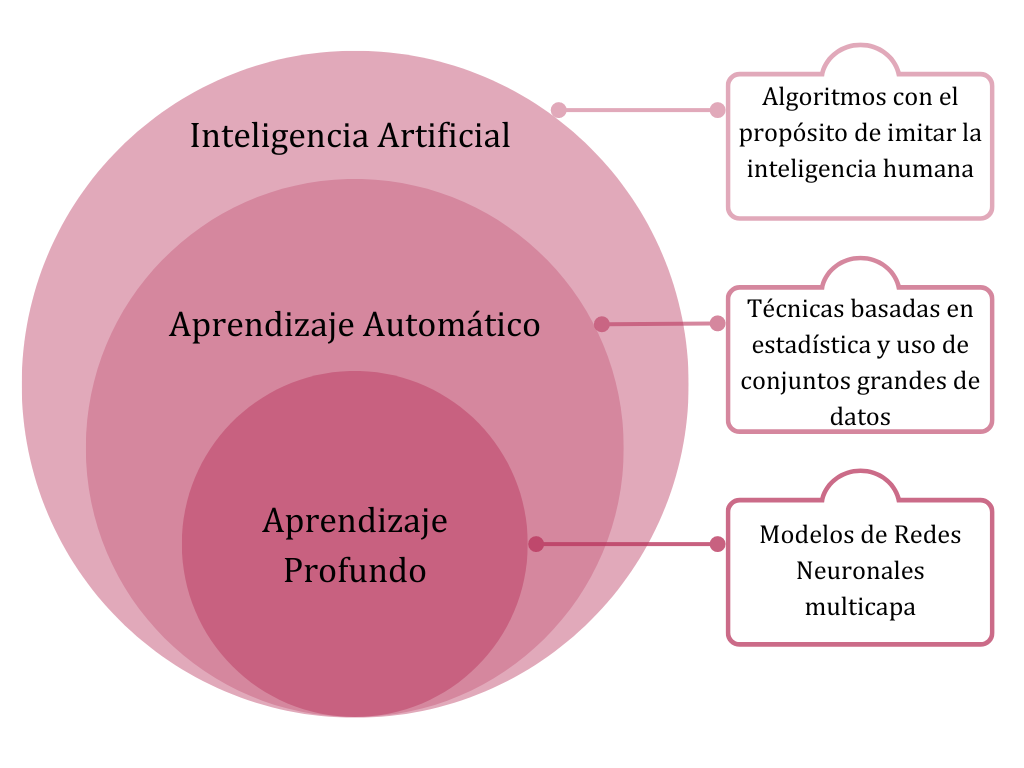
\includegraphics[width=0.7\textwidth]{/home/jessica/Tesis/img/tesis/IA_ML_DL.png}
  \caption{Diagrama de Venn que muestra los conceptos de Inteligencia Artificial, Aprendizaje Automático y Aprendizaje profundo.}
  \label{fig:IA-ML-DL}
\end{figure}

Los métodos de \textbf{Aprendizaje Automático} se pueden definir como un conjunto de métodos que pueden detectar automáticamente patrones en datos y aplicarlos para predecir nuevos datos. A grandes rasgos, los métodos de aprendizaje automático pueden dividirse en dos categorías: aprendizaje supervisado y aprendizaje no supervisado. \cite{murphy:2013}

\section{Aprendizaje Supervisado}
En el \textbf{aprendizaje supervisado} el objetivo es aprender, a partir de un conjunto de $M$ datos de entrenamiento definidos como:
\begin{equation}
\{\vec{x}_i, y_i\}_{i=1}^{M}
\end{equation}
una forma de mapear $\vec{x}_i$ a $y_i$.
\\
Cada vector:
\begin{equation}
\vec{x}_i = (x_1,x_2, \dots , x_d)_i\label{eq:trainset}
\end{equation}
corresponde a un dato, en donde cada componente es una \textbf{caracteristica} o \textbf{atributo} del dato en cuestión, y el número de componentes depende del problema. Algunos ejemplos de $\vec{x}_i$ son:
\begin{itemize}[label=\textcolor{CTtitle}{\textbullet}]
\item Imágenes
\item Enunciados de texto
\item Audios de voz
\item Series de tiempo
\end{itemize}

Por otro lado, $y_i$ corresponde a la \textbf{etiqueta} de $\vec{x}_i$. Cuando $y_i$ puede tomar un valor categórico, es decir, que de un conjunto finito:
$$y_i \in \{1,\dots,c\}, \text{  por ejemplo: 1=perro, 2=gato, etc. }$$ 
se dice que se trata de un problema de \textbf{clasificación}. Por otro lado, si $y_i$\footnote{$y_i$ puede ser también un vector: $\vec{y}_i$, en donde su dimensión está determinada por el problema a resolver, y no necesariamente es igual a la de $\vec{x}_i$.} es un valor real, se dice que el problema es de \textbf{regresión}.
\\

Algunos ejemplos de métodos de aprendizaje supervisado son:
\begin{itemize}[label=\textcolor{CTtitle}{\textbullet}]
\item Árboles de desición: Para problemas de clasificación
\item Regresión lineal: Para problemas de regresión
\item Redes Neuronales: Para problemas de regresión y de clasificación
\end{itemize}

\section{Aprendizaje No Supervisado}
En el \textbf{Aprendizaje No Supervisado} el conjunto de entrenamiento de $M$ datos se reduce a:
\[ \{\vec{x}_i\}_{i=1}^M \]
en donde no se cuenta con una etiqueta $y_i$. En este tipo de problemas, los métodos están enfocados en buscar patrones importantes a partir de únicamente los datos de entrada.
\\
Algunos ejemplos de métodos de aprendizaje no supervisado son:
\begin{itemize}[label=\textcolor{CTtitle}{\textbullet}]
\item Clustering: Agrupar datos similares entre sí
\item Análisis de Componentes Principales: Buscar la relación entre las caracteristica de los datos y reducir su dimensionalidad
\end{itemize}





